The focus is on the security aspects of autonomous on-roar motor vehicles,
in particular the cybersecurity threats, standards, and industry practices used to secure these systems.
This review will not cover the ethical implications or the differences between human-driven and autonomous vehicles in terms of accidents and fatalities.

\subsection{Historical roots}\label{subsec:historical-roots}

The development of autonomous vehicles is a significant milestone in the evolution of intelligent transport systems.
It is important to start with some historical context to understand the current state of autonomous vehicles and then,
the security implications.

Vehicle automation has roots dating back to 1918 (Pendleton et al., 2017),
with General Motors showcasing the first concept of an automated vehicle in 1939 (Shladover, 2018).
Initial R\&D efforts were led by General Motors and the Radio Corporation of America Sarnoff Laboratory in the 1950s
(Shladover, 2018).
From 1964 to 2003, various government and academic initiatives in the US, Europe,
and Japan focused on automated buses, truck platoons, and advanced driving systems
(Shladover, 2018).
A significant boost came from DARPA’s Grand Challenges Program in the 2000s \cite{darpa_grand_challenges_book},
where AVs first navigated desert terrains in 2005 and urban roads by 2007 (Pendleton et al., 2017; Shladover, 2018).

Since then, researchers have rapidly progressed in academia and industry.
Volvo, Tesla, Audi, BMW,
Mercedes-Benz and Nissan are some of the major car manufacturers that have invested in AV technology \cite{faisal2019understanding}.

\begin{figure}[!htb]
    \centering
    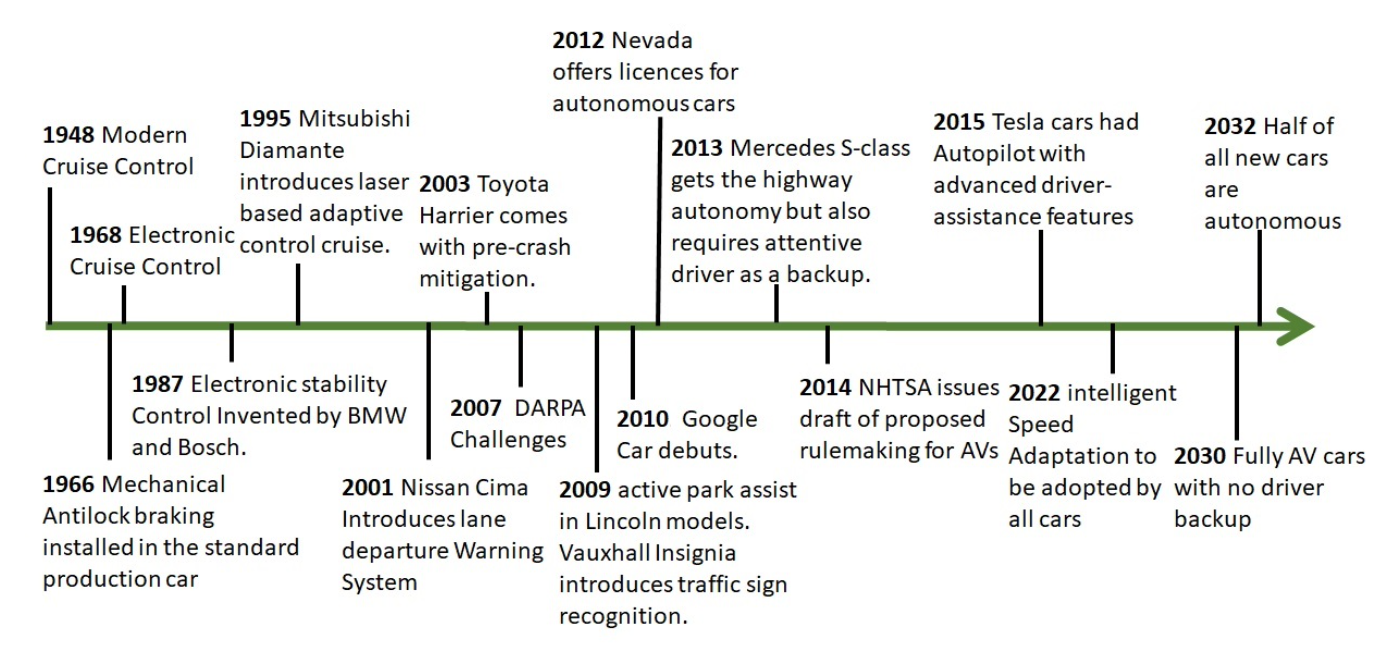
\includegraphics[width=0.7\linewidth]{figures/history}
    \caption{Historical timeline of autonomous vehicles.}
    \footnotesize{From \cite{ahangar2021survey} }
    \label{fig:history}
\end{figure}

\subsection{Autonomous Vehicles}\label{subsec:autonomous-vehicles}

As key parts of cyber-physical systems (CPS), vehicles are expected to effectively address current automotive challenges.
The shift towards vehicle-to-everything (V2X) in future mobility increases the complexity of security issues, particularly in terms of adaptability, dynamism, and self-awareness \cite{connected_vehicles_security_2023,bouchouia2023survey} .
While there have been notable advancements in security for intelligent mobility, the transition from static security approaches remains necessary.
For instance, vehicles relying on open software protocols and connecting with in-vehicle electric infrastructures play a vital role in strengthening their security framework.
With the integration of advanced sensor platforms, these vehicles essentially evolve into highly sophisticated seto of technologies influencing each other.
This transformation enables capabilities such as in-vehicle computing, fleet management, synchronization, telemetry, and seamless information sharing in urban mobility settings. CITAZIONE
Additionally, these vehicles will manage network traffic transactions through embedded systems.
Given their capabilities, connected, intelligent, and autonomous vehicles not only generate vast amounts of data but also function as mobile virtual data sources and intelligent mobile entities.


\subsection{Overview of AVs Architecture}\label{subsec:overview-on-avs-architecture}

This section provides an overview of the architecture of autonomous vehicles (AVs) and the key parts that enable their operation.
Moreover, an alternative architecture proposed in \cite{2023survey} will be briefly discussed.
The architecture of AVs is designed to integrate various hardware and software components that work together to perceive the environment, make decisions, and control the vehicle.

\cite{architecture}

\begin{figure}[!htb]
    \centering
    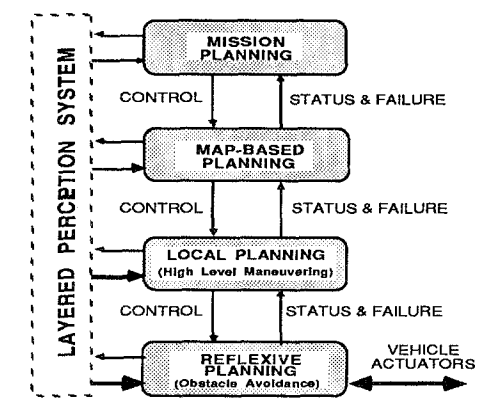
\includegraphics[width=0.7\linewidth]{figures/state-architecture}
    \caption{Hierarchical architecture of autonomous vehicles control.}
    \footnotesize{From \cite{architecture} }
    \label{fig:architecture}
\end{figure}

The current architecture is composed of layers of hardware and software that interact to enable the vehicle to operate autonomously.
In its simplest form, the architecture consists of three main layers: communication, security, network and components layer.

The proposed architecture extends the state-of-the-art providing four new components: monitoring, analysis, decision-making, and visualization.
Any services, processes, and communication are monitored
by the agents and analyzed by the process controllers.
A set of decision controllers act
on the information from the process controllers.
The decisions are archived in the black
box, while the analysis, report, and visualization layers are capable of both in-vehicle and
external virtual security operation center (VSOC) HMIs.


\subsubsection{Levels of Automation}\label{subsubsec:levels-of-automation}
The level of driving automation is determined by the specific roles assigned to both the driving automation system feature and the human user in performing the dynamic driving task (DDT) and DDT fallback. \cite{sae_j3016_2021}
The manufacturer of the automation system defines the requirements, operational design domain (ODD), and operating characteristics of the feature, including its level of automation.
Additionally, the manufacturer outlines how the feature should be properly used, ensuring that its capabilities and limitations are clearly understood and followed during operation.
The Society of Automotive Engineers (SAE) has defined six levels of driving automation, ranging from no automation (Level 0) to full automation (Level 5) \cite{sae_j3016_2021}.

\begin{enumerate}
    \item \textbf{Level 0 (No Automation):} The human driver is responsible for all aspects of the dynamic driving task.
    \item \textbf{Level 1 (Driver Assistance):} The vehicle assists the driver with specific tasks, such as steering or acceleration.
    \item \textbf{Level 2 (Partial Automation):} The vehicle can control both steering and acceleration/deceleration simultaneously under certain conditions, but the driver must remain engaged and monitor the environment.
    \item \textbf{Level 3 (Conditional Automation):} The vehicle can perform all aspects of the DDT under certain conditions like in traffic jams or highway driving, but the driver must be ready to take over when prompted.
    \item \textbf{Level 4 (High Automation):} The user (become passenger) does not need to supervise the Automated driving system (ADS) or be receptive to a request to intervene while the
    ADS is engaged, restricted to some conditions (e.g. Google's Self-Driving Car \cite{teoh2017rage}).
    \item \textbf{Level 5 (Full Automation):} The vehicle can perform all aspects of the DDT under all conditions without human intervention.
\end{enumerate}

\begin{table}[ht]
    \centering
    \begin{tabular}{|c|l|}
        \hline
        \textbf{Acronym} & \textbf{Definition} \\ \hline
        ADS & Automated Driving System \\ \hline
        DDT & Dynamic Driving Task \\ \hline
        ODD & Operational Design Domain \\ \hline
        OEDR & Object and Event Detection and Response \\ \hline
    \end{tabular}
    \caption{Definitions of Key Acronyms in Automated Driving}
    \label{tab:acronyms}
\end{table}

Levels 0–2 are generally classified as driver-assisted systems, while Levels 3 and 4 are considered semi-automated, and Level 5 represents full autonomy.

\subsubsection{Communication}\label{subsubsec:communication}

Communications are essential for AVs to interact with other vehicles, infrastructure, and the cloud.
When speaking about communications in the AVs context, it is important to consider and scind the communication type in different categories:
\begin{enumerate}
    \item Vehicle-to-vehicle (V2V): communication between vehicles
    \item Vehicle-to-infrastructure (V2I): communication between vehicles and infrastructure, such as traffic lights and road signs
    \item Vehicle-to-pedestrian (V2P): communication between vehicles and pedestrians, such as smartphones or wearables to improve security (not in terms of cybersecurity)
    \item Vehicle-to-network (V2N):
    \item Vehicle-to-cloud (V2C)
\end{enumerate}


\subsubsection{Perception}\label{subsubsec:perception}
It is fundamental in AVs to perceive the environment and understand the context in which the vehicle is operating for obvious reasons.
The perception system is responsible for collecting data from various sensors, such as cameras, LiDAR, radar, and ultrasonic sensors, to create a detailed representation of the vehicle's surroundings.
In this case, it is important to consider the possible tempering that can be done on this sensors to alterate the perception of the vehicle, leading to dangerous situations.

\subsection{Cyber-insecurity consequences}\label{subsec:cyber-insecurity}

Before introducing new threats of new autonomous vehicle technologies, it is important to understand the current state of cybersecurity in AVs and some historical key attacks.
In the past, researchers have demonstrated various attacks on AVs, including remote hijacking, sensor spoofing, and data breaches.
As specified in \cite{cybersec} the attack surface of AVs is expanding due to the increasing complexity of these systems, which rely on a combination of hardware, software, and communication technologies.
This expansion is due to the aggressive attempts of automakers to
make vehicles fully autonomous in a short period of time and without considering the security implications.
This implied a lot of new technologies and new communication protocols keeping the focus always on the functionalities offered to the driver in terms of comfort.
The security of the vehicle has been considered as a secondary aspect, leading to a lot of vulnerabilities that can be exploited by attackers.

Attackers can exploit these vulnerabilities to compromise the safety and functionality of AVs, posing significant risks to passengers, pedestrians, and other road users.
Since now cars are connected to the internet, there is no need to be physically close to the car to exploit these vulnerabilities and this expands the attack surface drastically.
In the past decade (2010 onward), nearly 79.6\% of all automotive attacks have been
remote attacks.

Some famous attacks that bring the attention to the security of AVs are:
\begin{enumerate}
    \item The Jeep Cherokee hack in 2015, where researchers remotely hijacked a Jeep Cherokee through its infotainment system, demonstrating the potential risks of cyber-attacks on connected vehicles \cite{miller2015remote} .
    \item The Tesla Model S hack in 2016, where researchers exploited vulnerabilities in the vehicle's software to take control of the car's brakes, door locks, and other critical systems \cite{tesla_hack}.
    \item The Nissan Leaf hack in 2016, where researchers demonstrated how an attacker could remotely control the vehicle's heating and air conditioning systems, drain the battery, and access the driver's personal information.
    \item The VW group hack in 2016, where researchers discovered vulnerabilities in the keyless entry systems of several VW group vehicles, allowing attackers to unlock the doors and start the engine without the key fob \cite{garcia2016lock}.
\item \end{enumerate}

These are only some examples of the potential risks associated with AVs and the need for robust cybersecurity measures to protect against cyber-attacks.
One of the latest is the Tesla cybertruck vulnerabilities that have and continue to be exploited by attackers to gain access to the vehicle's systems and control its functions remotely.



























New sensing and communication capabilities bring the Autonomous vehicle to eexpose a big attack surface  \cite{unknown2020connected}
\cite{cybersec}

\subsection{Motivation}\label{subsec:motivation}

\subsection{Social implications}\label{subsec:social-implications}

This section aims to provide a little insight into the social implications of autonomous vehicles.
The introduction of autonomous vehicles (AVs) is expected to have a profound impact on society \cite{thomas2020perception}, transforming transportation systems \cite{intelligent_transportation_2023}
, urban planning \cite{impact_autonomous_vehicles_2018}, and the economy \cite{economic_aspects_2020}.

\subsection{Structure of the Survey}\label{subsec:structure-of-the-survey}
